% !TEX program = xelatex
\documentclass[sigconf,nonacm,anonymous,review]{acmart}

\usepackage{kotex}
\usepackage{graphicx}
\usepackage{booktabs}
\usepackage{array}
\usepackage{enumitem}
\usepackage{balance}
\usepackage{amsmath}
\usepackage{amssymb}
\usepackage{newunicodechar}
\usepackage{dblfloatfix}
\setlist[itemize]{leftmargin=*,nosep}
\settopmatter{printacmref=false, printccs=false, printfolios=true}
\renewcommand\footnotetextcopyrightpermission[1]{}
\pagestyle{plain}

% ---- unicode symbols used in the Korean body (xelatex) ----
\newunicodechar{→}{\ensuremath{\rightarrow}}
\newunicodechar{↔}{\ensuremath{\leftrightarrow}}
\newunicodechar{≤}{\ensuremath{\le}}
\newunicodechar{≥}{\ensuremath{\ge}}
\newunicodechar{≈}{\ensuremath{\approx}}
\newunicodechar{×}{\ensuremath{\times}}
\newunicodechar{∈}{\ensuremath{\in}}
\newunicodechar{±}{\ensuremath{\pm}}
\newunicodechar{·}{\textperiodcentered}
\newunicodechar{°}{\textdegree}
\newunicodechar{τ}{\ensuremath{\tau}}
\newunicodechar{✓}{\ensuremath{\checkmark}}
\newunicodechar{✗}{\ensuremath{\times}}
\newunicodechar{⓪}{(0)}
\newunicodechar{①}{(1)}
\newunicodechar{②}{(2)}
\newunicodechar{③}{(3)}
\newunicodechar{④}{(4)}
\newunicodechar{⑤}{(5)}
\newunicodechar{⑥}{(6)}
\newunicodechar{⑦}{(7)}

% placeholder box for figures whose plots are deferred this round
\newcommand{\figtodo}[1]{\fbox{\parbox[c][2.6cm][c]{.92\linewidth}{\centering\itshape #1\\[3pt]\normalfont\footnotesize[\,placeholder: plot inserted once measurements are in\,]}}}

\title{OVLA: On-device Verification of LLM-Generated IoT Automations via Timeline IR}
\author{Anonymous Submission}
\affiliation{\institution{Submitted to SenSys 2027}\country{}}
\email{}

\begin{document}

\begin{abstract}
Smart home automation increasingly relies on Large Language Models (LLMs) to translate natural language (NL) user intents into executable reactive rules. However, deploying these rules directly on edge hubs poses severe reliability and safety risks since reactive IoT automations are temporally complex, involving precise triggers, durations, and repetitions. Existing validation methods rely heavily on human code inspection, offline experts, or resource-heavy cloud LLM re-checks, failing edge privacy and latency constraints. To tackle this challenge, we present OVLA, an on-device pipeline for deterministic, LLM-free verification of IoT automations before deployment. OVLA bridges the gap between informal natural language and strict execution using Timeline IR, a compact, machine-checkable representation of temporal behavior. The pipeline first translates the user's NL intent into a typed Timeline IR; the user confirms a deterministic plain-language rendering of this IR, which then serves as the reference specification of the intended behavior. OVLA then automatically synthesizes reference event traces and boundary cases from this IR. An efficient verifier simulates the generated rule code against these traces to detect behavioral discrepancies and guide automated repairs via counterexamples. Evaluated with a local, quantized ≤9B model across 382 automations, OVLA caught every faulty program in our evaluation set, repairing 31\% of them and rejecting the rest fail-closed. Under 1,552 injected temporal bugs, it detected 99.3\%, while its synthesized scenarios exercised 97.5\% of specification-side obligations and 97.7\% of generated-code branches, raising the share of correctly deployed automations from 90.8\% to 93.7\%, all without any LLM in the verification loop.
\end{abstract}

\keywords{IoT automation, LLM code generation, reactive-temporal code, deterministic verification, on-device, trace equivalence}

\maketitle

\section{Introduction}

IoT automation is rapidly moving toward LLM-based code generation. A user states the desired behavior in natural language, and an LLM turns it into a reactive rule the platform can execute. Yet the final step of this workflow, deciding \emph{whether the generated code is correct to deploy}, has no deterministic gate. The missing piece is a reference to check the code against; the natural-language request contains the intent, but not in a form that can serve as a rigorous baseline for automated testing.

\textbf{Why this is hard:} The core challenge stems from the absence of a verifiable reference baseline. The target automations are inherently \emph{reactive-temporal}. They are \emph{reactive} because their execution is driven by asynchronous events and conditional triggers,
and \emph{temporal} because their behavior unfolds over time through schedules, periodic executions, and sustained state durations (e.g. ``if it persists for more than N minutes'').
Driven by timers, counters, and multi-step state, the correct behavior of an automation must be evaluated across an entire timeline rather than a single discrete instant. Furthermore, in our setting, this logic is deployed as arbitrary code rather than a restricted, fixed-rule template.
Validating their correctness presents two key challenges. First, no test oracle is available. 
Unlike text-to-SQL or traditional programming benchmarks that supply gold denotations or input-output test suites, a reactive automation's output is a future sequence of environment interactions. Because no external source can pre-label this sequence, the verification reference must be actively constructed on the fly. 
Second, syntactic divergence complicates evaluation. The same user intent can be expressed through many syntactically different yet behaviorally equivalent implementations. Therefore, checking a generated program by matching it against any single reference text is neither sound nor complete. Determining correctness fundamentally requires reasoning about the program’s semantic behavior over time, rather than analyzing its static syntax or a single snapshot of its output.

\textbf{Running example:} Suppose a user requests ``whenever the temperature rises above 25°C, turn on the air conditioner.'' We read ``rises above'' as an edge-triggered intent: the AC should be switched on once per upward crossing, not continuously while it stays hot. Figure~\ref{fig:idiom} shows three lowerings, sketched in JoI, the automation DSL of our target platform (\S4). Implementation (a) detects the crossing by comparing the previous and current temperature readings while (b) keeps a flag that is set on firing and reset when the temperature falls back below the threshold. (a) and (b) share almost nothing syntactically yet behave identically, so no syntactic comparison can certify one against the other. Implementation (c) appears to be the most intuitive translation because it textually mirrors the natural-language request. However, it is the wrong one: under periodic execution it falsely re-fires on every tick as long as the temperature stays above the threshold. All three are syntactically valid and look plausible; they can only be differentiated by evaluating their execution traces over time; because repeated On() commands leave the AC in the same visible state, the user may see nothing wrong. This is a crucial failure mode our system eliminates: \textbf{deployed code that silently diverges from the user's intended behavioral specification}. (In the sketches, \texttt{cron} sets when the script starts, \texttt{period} is the tick interval in milliseconds, and \texttt{code} is the body executed on every tick; \texttt{:=} initializes a persistent variable once, while \texttt{=} performs per-tick update.)

\begin{figure}[t]
\centering

\includegraphics[width=\linewidth]{figs/figure1_a.pdf}\par
{\small (a) Previous/current comparison}\par\smallskip
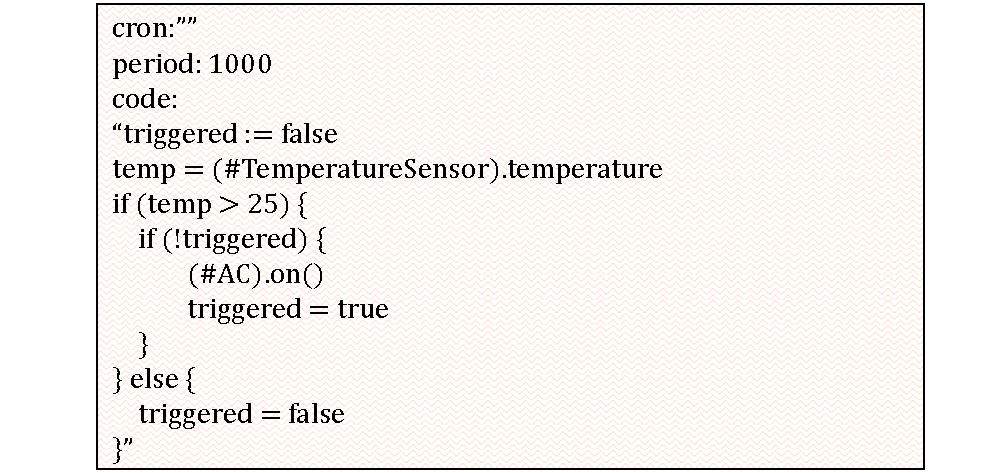
\includegraphics[width=\linewidth]{figs/figure1_b.pdf}\par
{\small (b) Triggered flag}\par\smallskip

\includegraphics[width=\linewidth]{figs/figure1_c.pdf}\par
{\small (c) Re-fires while the level holds}\par\smallskip
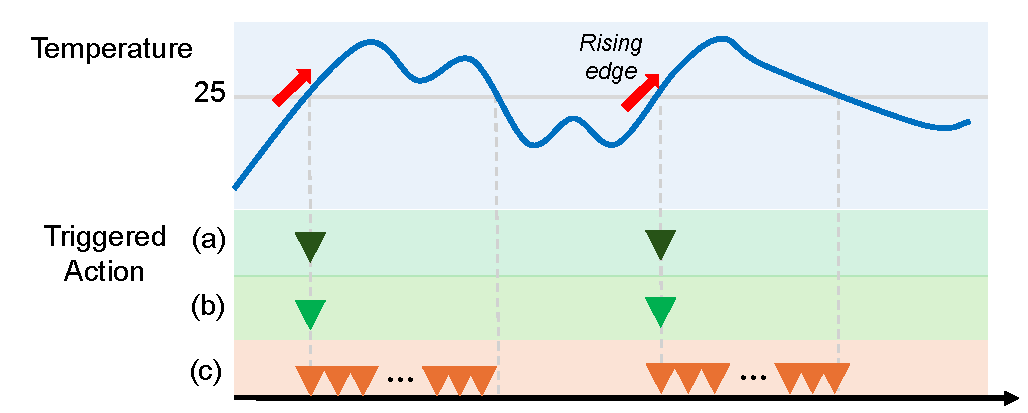
\includegraphics[width=\linewidth]{figs/figure1_trace.pdf}\par
{\small (d) Action traces}
\caption{Three lowering sketches of one intent (``whenever the temperature rises above 25°C, turn on the air conditioner'') and their action traces. (a) and (b) produce identical traces; (c) fires on every tick while the threshold is exceeded.}
\label{fig:idiom}
\end{figure}

\textbf{Why existing checks fall short.}
Prior verification frameworks of IoT automations target fixed, predefined criteria rather than the user's intent. A large body of work checks hand-authored trigger-action rules; for instance model checkers prove safety properties, inter-rule conflicts, or security policies (e.g., AutoTap~\cite{autotap}), while runtime monitors flag deviations from mined invariants~\cite{hawatcher}. This limitation is a consequence of design paradigm, not oversight. When a user writes the rule directly, the rule itself serves as the ground-truth intent, and critical risks worth verifying, such as rule conflicts and security violations, can be defined, without referencing the unique intended behavior of a specific task.
However, as the user transitions from author to prompter, the verification paradigm fundamentally changes. Once an LLM synthesizes code from a natural-language request, the user’s original statement and the generated artifact become distinct, decoupled entities that can silently diverge. In this generative workflow intent-conformance emerge as a critical, unaddressed checkpoint.

In that generation setting, the gap remains wide open, and bridging it hinges on a single question:
does a test oracle already exist? Generators designed for algorithmic IoT code can readily validate their output against executable test suites or labeled accuracy, similar to how text-to-SQL frameworks verify relational denotations. For these domains, intent-conformance is effectively a solved problem (e.g., GPIoT~\cite{gpiot}). Reactive automations, however, lack any such ready-made oracle. Hence natural language-to-automation generators must settle for weaker proxies: schema validity (e.g., verifying that the framework accepts the JSON syntax), device grounding feasibility, lexical matching against ground-truth commands, or evaluation by an LLM judge. Even frameworks that present the generated rule back to the user rely on manual, error-prone human-in-the-loop confirmation rather than formal verification of the underlying executable code (e.g., AwareAuto [16]). To date, no existing system deterministically verifies that reactive-temporal code faithfully executes the user's behavioral intent over time. The fundamental missing piece is not a more capable language model, but a verifiable reference specification.

\textbf{Why not an LLM judge.} The remaining alternative that targets user intent directly is to ask another LLM whether the code matches the request. But an LLM judge is too unstable to act as a deployment gate. A deployment decision is binary: two behaviorally identical programs must receive the same deploy/reject verdict. Yet we find that on behavior-preserving programs that differ only in idiom, an LLM judge's verdict flips even at temperature 0 (\S3). Larger models still flip, and cloud models violate the privacy and latency constraints of the edge. A gate whose verdict tracks the surface form of the code is not fit to gate deployment.

\textbf{OVLA.} To address these challenges, we present OVLA. Its key idea is to \emph{derive the missing reference specification} at authoring time and subsequently utilize it as a deterministic verification baseline.
First, OVLA builds a candidate Timeline IR from a natural-language request. Then, the system generates a deterministic, plain-language rendering of this IR for the user to review and confirm.
This confirmed IR serves as a per-automation behavioral oracle. The generated JoI code is then verified against the oracle by bounded trace-equivalence over the finite set of transition points defined by the IR. Both components are run on events synthesized at those points (e.g., timer expirations, condition thresholds, and cycle restarts), and their resulting action traces are compared. While the LLM is confined to \emph{generation}, proposing the IR and lowering it to code, both the rendering step and the equivalence check are deterministic and LLM-free. This allows conformant automations to be safely deployed at the edge without cloud-side review. \emph{Precisely because} lowering relies on a probabilistic LLM,
a deterministic checker is needed.

\textbf{Scope and assumptions.} 
OVLA targets natural-language commands specifying explicit reactive-temporal behaviors. Inferring intent from vague or affective goals (e.g., "make it cozy") is a separate intent-elicitation challenge addressed by orthogonal literature (e.g., Sasha~\cite{sasha}, SAGE~\cite{sage}) and is strictly out of scope. Any residual ambiguity within a specifiable command is intentionally surfaced by OVLA's deterministic rendering phase and resolved during user confirmation, rather than by the verifier itself. 
Confirming the IR is presented as a plain-language judgment rather than a programming task. The dimensions a user controls in reactive-temporal automation are limited and enumerable (start time, period, trigger and condition, action and its arguments, sustain and delay durations), Timeline IR expresses only these slots, and deterministic rendering displays them verbatim as a readable timeline (\S8.1). Approving an IR is thus a closed judgment over finite control slots the command named, not the authoring of arbitrary formal properties.

\textbf{Two-layer guarantee.} We explicitly define the boundaries of our verification scope.
In \textbf{Layer A (NL→IR)}, the system captures intent as IR and presents it in plain language, but we do not measure non-expert confirmation success \emph{itself} in this round via a human-subjects study (\S9). In \textbf{Layer B (IR→code)}, once the IR is approved, OVLA prevents the generated code from silently diverging from that displayed IR within a bounded behavior region. OVLA's technical guarantee lies firmly in Layer B.

\textbf{Deployment setting.} We assume a home edge device rather than the cloud, to ensure privacy (sensor data never leaves the home) and reduce latency.
This environment precludes a cloud LLM judge, requiring the validation gate to be an LLM-free deterministic check. Consequently, a single design decision simultaneously delivers trust (via a non-probabilistic judge) and deployability (millisecond-level localized execution with zero model-call overhead).

\medskip\noindent\textbf{Contributions.} 
To the best of our knowledge, OVLA is the first system for LLM-generated reactive-temporal IoT automations that transforms intent-conformance into a deterministic, pre-deployment verification check. It achieves this by establishing a user-confirmed behavioral IR as the authoritative test oracle, rather than relying on a probabilistic judge or superficial manual review.
\begin{itemize}
\item \textbf{C1. Timeline IR:} We introduce a unified representation that simultaneously serves dual roles:
(a) a surface that is deterministically rendered to plain language for user validation, and (b) a machine-checkable behavioral reference for validating reactive-temporal code. While an approved NL sentence can serve only (a) and a formal property only (b), our contribution lies in a singular representation that achieves both. Given that prior works can already generate confirmable temporal IRs, our distinct claim is the novel integration of deterministic, LLM-free verification, automatic rendering, and localized on-device operation
(\S2).
\item \textbf{C2. Deterministic deployment gate:} We propose an end-to-end pipeline, spanning IR→FSM→boundary event→bounded trace-equivalence, that executes entirely without LLM intervention. The gate operates under a fail-closed policy where a pass triggers immediate deployment and a failure triggers automatic repair or rejection.
When the gate rejects a program, it guarantees a genuine behavioral divergence under the defined observation model, ensuring rejection-soundness.
\item \textbf{C3. On-device realization:} The generation phase utilizes a 4-bit quantized model of at most 9 billion parameters without any fine-tuning, while the verification gate bypasses LLM execution entirely. Consequently, verification completes locally in about a millisecond at the median. OVLA's verification guarantee does not depend on the size or quality of the generation model.
\item \textbf{C4. Evaluation:} We evaluate rendering faithfulness (\S8.1) and verifier detection accuracy (\S8.2), empirically demonstrate system safety by mitigating silent IR-to-code divergence of 9.2\% down to zero (\S8.3), and measure on-device execution overheads and deployment feasibility (\S8.4) through rigorous component-by-component analysis.
\end{itemize}

\textbf{Focus of the contribution.} OVLA removes a failure mode that survives user approval: even when the approved IR is acceptable, the subsequent reactive-temporal lowering phase can introduce subtle state, timer, and boundary errors that cause the deployed code to diverge. OVLA serves as the deterministic, on-device gate specifically engineered to intercept and remediate exactly these errors.

\section{Related Work and Positioning}

Verification of home automations did not begin as an open problem. When users authored rules directly, the rule itself was the artifact under analysis, and formal techniques could check it against fixed properties; when code was generated in domains that ship executable tests, the tests served as the oracle. In both settings, a checkable reference existed before verification began. LLMs entered this workflow for a practical reason: authoring is the bottleneck, as end users struggle to write and debug even slot-based rules, and richer reactive-temporal behaviors require code they cannot write at all. This shift turns the user from an author into a prompter, separates the request from the artifact that implements it, and removes the very reference that earlier verification relied on. We therefore organize prior work by the reference each system checks against.

\textbf{When a verification reference already exists.} A rich body of work verifies hand-authored TAP rules with formal techniques. AutoTap~\cite{autotap} synthesizes or repairs TAP rules, modeled as transition systems, so that they satisfy LTL safety property templates chosen by the user. TAPInspector~\cite{tapinspector} model-checks timing-aware rule sets for safety and liveness violations and TAPFixer~\cite{tapfixer} repairs such violations; related analyses uncover inter-rule and security vulnerabilities~\cite{iruler,soteria}; and HAWatcher~\cite{hawatcher} monitors deployed automations against mined invariants at runtime. Deterministic verification is possible in this line because the reference is fixed in advance: a safety property, conflict freedom, or a security policy. Because the user authors the rule directly, the rule is itself the artifact under analysis, and a separate per-task intent reference is never required.

The same holds for generation targets whose domain supplies an executable oracle. GPIoT~\cite{gpiot} generates signal-processing and ML algorithm code from natural-language requirements using an on-device fine-tuned SLM and verifies the result with pass@k execution tests. Outside IoT, text-to-SQL verifies a generated query against the denotation of a gold query~\cite{spider}, and CodeT~\cite{codet} and Self-Debug~\cite{selfdebug} verify generated code with unit tests. \emph{Across both lines, verification was enabled by a checkable target that was already available, whether a fixed property, a test suite, or a gold denotation.}

\textbf{LLM-generated reactive automations: no ready-made reference.} LLM-generated reactive automations have no such target: the intended behavior is named only in the user's request, and no benchmark or test suite labels its future action sequence. The missing reference is also harder to substitute here than for TAP rules. TAP rules do carry temporal behavior, including triggers, stays-for durations, and cron-style schedules, but there it is a platform \emph{primitive}: the author fills slots and the engine implements the mechanism, so slot errors are visible on the face of the rule. In reactive-temporal code such as JoI scripts, no such primitive exists for edge detection, sustained conditions, or counting; the author, here an LLM, must realize the mechanism as an \emph{idiom} built from persistent variables, conditions, and per-tick execution. Mechanism errors are silent, and they are exactly where lowering bugs arise.

Some systems in this regime do check LLM output deterministically, but still against fixed criteria. AutoIoT~\cite{autoiot_maude} checks LLM-generated rules against four inter-rule conflict types using Maude rewriting logic. DS-IA~\cite{dsia} checks the device-grounding feasibility of a command with a deterministic cascade and rejects infeasible commands fail-closed before execution. TaskSense~\cite{tasksense} translates a sensing query into an executable tool-calling DAG, screens it with an LLM-based solvability check, and then deterministically checks that the plan's dependency graph is a subgraph of the toolset grammar; both checks establish structural well-formedness, and its only behavioral reference, a hand-authored ground-truth plan, exists solely in offline evaluation. AgentSpec~\cite{agentspec} enforces trigger-predicate safety rules on LLM agents at runtime through a deterministic DSL; however, its rules are fixed and hand-written rather than derived from the request being served. \emph{Most of these checks are deterministic, yet their reference remains a predefined criterion; the behavior the user actually asked for is still never the reference.}

Generation systems themselves fall back to weaker checks. ChatIoT~\cite{chatiot} translates natural language into Home Assistant automations with multiple LLM agents and has a separate ``Evaluator'' agent assess format compliance and request satisfaction; Giudici et al.~\cite{giudici2025} accept a generated routine if the framework parses its JSON; and IoTGPT~\cite{iotgpt} catches API violations and runtime errors, though not intent mismatches, in a virtual SmartThings environment. AwareAuto~\cite{awareauto} goes furthest: it builds a confirmable reactive-temporal rule with event/state modes, delays, branches, and sequencing, presents it to the user in a panel, and lowers it to executable JSON. \emph{Across this line, automatic checking stops at format adequacy, API validity, or device-grounding feasibility. Even in AwareAuto, intent consistency is evaluated through researcher annotation, and the user-facing confirmation text is generated prose rather than a deterministic rendering. Consequently, none of these systems verifies that the generated code behaves as the user intended.}

Work that directly asks whether the generated artifact matches the user's intent remains rare. LACE~\cite{lace} back-translates a generated access-control policy into natural language with deterministic templates and judges semantic equivalence against the original request with a fine-tuned NLI model. SimuHome~\cite{simuhome} judges agent behavior against goal states in a time-accelerated simulator and shows that 18 LLM agents largely fail to self-correct their own reactive-temporal errors (\S3); its goals, however, are authored by the benchmark rather than confirmed by a user, and it evaluates agents rather than gating deployment. \emph{Even where intent is addressed directly, intent has no ground truth other than the user, so a model-only verdict certifies itself, as in LACE's reported ``100\% correctness''.}

Two systems come nearest to OVLA, each along one axis of our problem: LACE on the reference axis, since it checks a generated artifact against the user's request, and AwareAuto on the artifact axis, since it builds a confirmable reactive-temporal representation. LACE, however, judges probabilistically over static policies, and AwareAuto never verifies the behavior of the lowered code. OVLA starts precisely where both stop, treating the user as the only legitimate source of the reference: it derives the missing reference at authoring time, takes the user-confirmed IR as the behavioral oracle, and checks the generated reactive-temporal code through deterministic, LLM-free trace-equivalence, before deployment and on the device. We note that merely combining generation with verification is standard practice in this field and is not our claimed novelty; the novelty lies in the combination of a user-confirmed behavioral reference, deterministic LLM-free checking, and on-device operation, which no single prior system provides together.

\section{Problem and Motivation}

Together, \S1 and \S2 leave a clear task: a gate is needed that decides, before deployment, whether LLM-generated reactive-temporal code behaves as the user intended. This section first establishes the requirements such a gate must meet in our setting. Next it weighs alternative candidate checking approaches against them, and finally measures the one remaining candidate, an LLM judge, motivating our proposed solution.

\textbf{Three requirements for a deployment gate.}
\begin{itemize}
\item \textbf{R1 (Reference).} No prior reference exists. The intended behavior is determined solely by the user’s recent request, meaning it is not provided as a checkable artifact.
Algorithmic code carries an executable oracle in the form of input-output pairs and is checked by running tests (GPIoT~\cite{gpiot}, \S2). For reactive-temporal code, the ``right output'' is a future sequence of device actions that no external source labels. The reference must be constructed, not looked up.
\item \textbf{R2 (Stability).} A deployment decision is binary: two programs with the same behavior must receive the same deploy/reject verdict. A checker whose verdict wavers under behavior-preserving rewrites is unsuitable as a gate, regardless of the quality of its individual judgments.
\item \textbf{R3 (On-device).} Sensor data must not leave the home (privacy) and the verdict must be immediate (latency), so the gate must run on the edge without a cloud round-trip.
\end{itemize}

\textbf{Candidate 1: syntactic or structural comparison.} The most straightforward verification method is to match the generated code directly against a reference text. However, as demonstrated by the temperature control example in \S1 (Figure~\ref{fig:idiom}), identical user intent can be realized through syntactically disparate idioms (a prev/curr comparison vs.\ a triggered flag), while the buggy implementation is the one that most resembles the request. Indeed, near-miss bugs differing by only a single execution tick or a single comparison can appear identical to valid code variants. Because syntactic or structural matching can neither validate diverse correct variants nor isolate subtle bugs, it satisfies neither soundness nor completeness.
Equivalence must be decided on execution behavior, not on syntax.

\textbf{Candidate 2: self-checking by the generating model.} One could ask the model that produced the code to inspect and repair it. SimuHome~\cite{simuhome} evaluated this method with 18 models; the self-correction recovery rate was 8.0\% for time-based errors, 18.5\% for event-based errors, and 0.0\% for coordinated scheduling. Notably, the success rate remained at or below 67\% even when an oracle was provided. Based on these findings, the authors concluded that agents fail to detect flaws in their own plans. A post-hoc self-check entrusted to the same stochastic process that generated the code cannot serve as a reliable quality gate.

\textbf{Candidate 3: human inspection of the code.} One could show the generated code to the user for approval. However, prior research in TAP-Debug~\cite{tapdebug} demonstrated that non-experts frequently misread even the basic IF (event) and WHILE (state) conditions of raw rules; specifically, misreadings occurred in 21 out of 50 control-condition sessions, all of which subsequently failed the task. Given that such errors occur even with a simple, two-slot TAP rule, it is untenable to expect users to successfully inspect complex reactive-temporal code, which realizes its mechanism through persistent variables and per-tick execution. What is shown to the user must be a readable representation rather than the raw code; this also motivates the deterministic rendering detailed in \S5.

\textbf{The remaining candidate: an LLM judge.} What remains is to hand the request and the code to a separate LLM to verify whether they align. This approach appears plausible at first glance and is indeed used in practice (ChatIoT's Evaluator, \S2), and existing literature does not rule it out. We therefore evaluate whether this candidate meets R2 independent of OVLA's IR and verifier.

We presented pairs of programs exhibiting identical behavior (trace-exact) but differing in idiom, and measured how often the judge's accept/reject verdict flipped. Even under a deterministic setting at temperature 0, a 9B model flipped on 27\% of pairs and a strong cloud-based model flipped on 10.6\%. The rewrite types are categorized into surface rewrites (SEL = selector order, AND = $A{\wedge}B{\leftrightarrow}B{\wedge}A$, VAR = variable renaming) and logic/arithmetic rewrites (ADD = $x{+}n{\leftrightarrow}n{+}x$, BR = branch swap, DN = double negation, DM = De Morgan, IDM = idiom replacement). As shown in Figure~\ref{fig:instability}, purely surface rewrites flipped up to 9\% of the 9B judge's verdicts (14\% for the cloud judge), while logic and arithmetic rewrites caused flips up to 81\%. No ground-truth label is required to demonstrate this; the flip itself evidences instability.

The core is not the miss rate; on cleanly injected bugs, strong models are indeed competent detectors. The point is that \emph{any} probabilistic judge yields an unstable deployment policy under behavior-preserving rewrites. This instability persists in larger models, and majority voting fails to reduce it below the temperature-0 baseline, because voting mitigates sampling noise but cannot counteract the systematic dependence on surface form (Table~\ref{tab:instab}). This violates R2, disqualifying the final candidate. In contrast, OVLA's verdict depends only on behavior over a bounded set of traces, so under the same rewrites its flip rate is 0 by construction.

\begin{figure}[t]
\centering
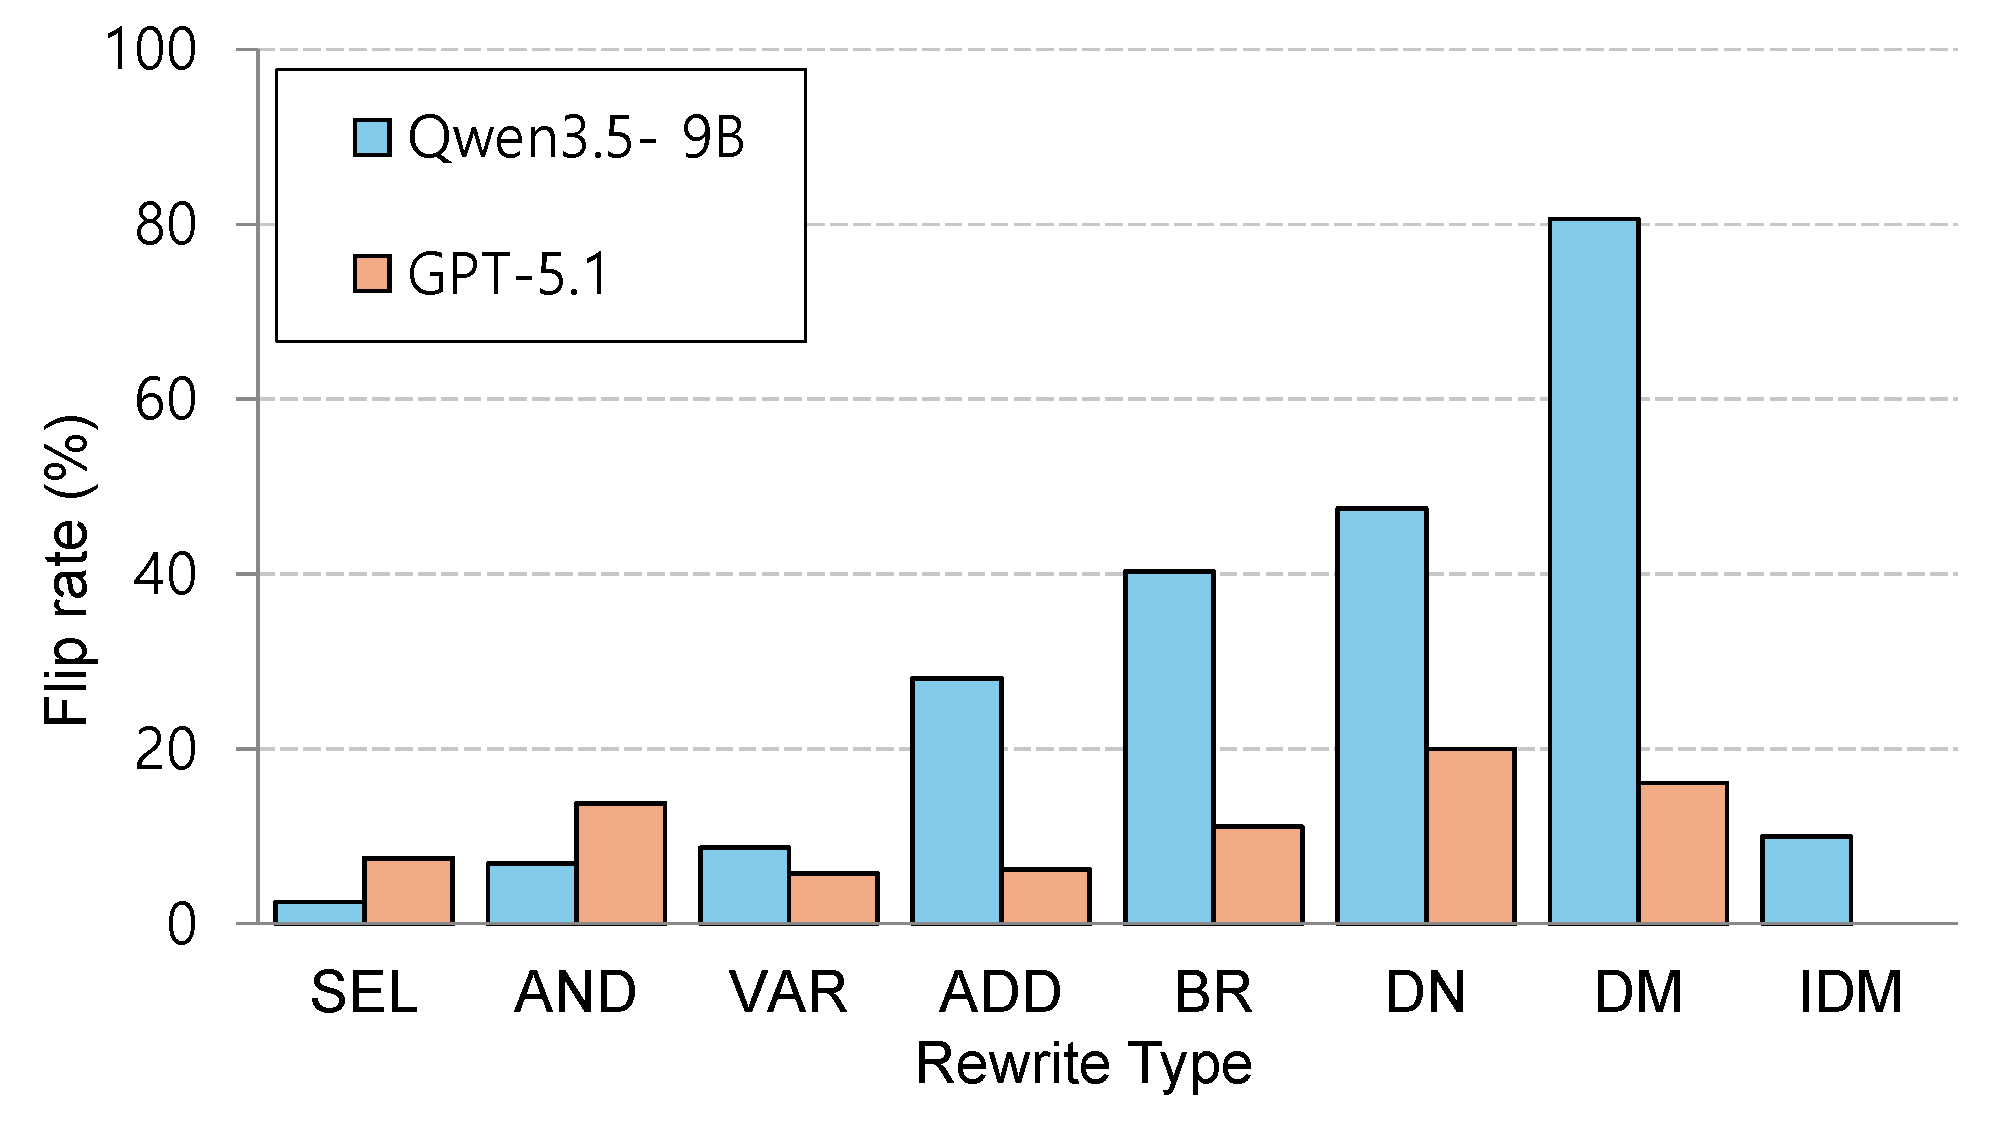
\includegraphics[width=\linewidth]{figs/instability.pdf}
\caption{LLM judge verdict flip rate by rewrite type on behavior-identical programs (temperature 0).}
\label{fig:instability}
\end{figure}

\begin{table}[t]
\centering
\caption{Overall flip rate by judge configuration; OVLA's trace check flips on none of the same rewrites.}
\label{tab:instab}
\begin{tabular}{lcc}
\toprule
Judge configuration & 9B & GPT-5.1 \\
\midrule
deterministic (temp=0) & 27.0\% & 10.6\% \\
+ sampling (temp=0.7) & 34.4\% & 12.8\% \\
+ majority vote (K=5) & 31.2\% & 13.5\% \\
\textbf{OVLA (deterministic trace)} & \textbf{0\%} & \textbf{0\%} \\
\bottomrule
\end{tabular}
\end{table}

\textbf{The surviving design.} With every candidate eliminated, rereading the requirements reveals the shape of the answer. By R1, the reference must be \emph{derived} from intent the user has confirmed; by R2, the check must be deterministic over behavior (traces), not syntax; by R3, it must be lightweight on the edge, with no LLM call. The artifact that satisfies all three at once is the Timeline IR (\S5), and the deterministic trace-equivalence check over it is the verifier (\S6). The judge in this motivating experiment compares NL against code.

\begin{figure*}[t]
\centering

\includegraphics[width=\textwidth]{figs/system.pdf}
\caption{OVLA system overview. ①{--}⑤ Generation phase and ⑥{--}⑦ verification phase; the dashed arrow is the counterexample-guided repair loop.}
\label{fig:arch}
\end{figure*}

\section{System Overview}

OVLA implements the aforementioned design as a two-phase pipeline. In the authoring phase, the system derives a Timeline IR from the user's command, renders that IR for confirmation, and lowers the confirmed IR to executable code. In the verification phase, the system checks the generated code against the confirmed IR before deployment. The central boundary is fixed throughout the pipeline: the LLM may propose candidate artifacts, but every artifact that can affect deployment is checked by deterministic code.

\textbf{Execution target.} We instantiate OVLA on the edge hub of a commercial IoT platform whose execution DSL is JoI. A JoI automation consists of a start schedule (\texttt{cron}), a re-execution interval (\texttt{period}), and a script body (\texttt{code}). When the \texttt{period} parameter is positive, the body is executed on each tick, and temporal behavior such as edge detection, sustained conditions, and counting must be implemented with persistent variables and ordinary conditionals. JoI therefore serves as the executable artifact produced by the lowering phase as well as the primary artifact checked by the verifier.

Figure~\ref{fig:arch} shows the complete pipeline. The first phase, authoring, includes LLM-based generation steps and deterministic gates that execute before the user approves the reference. The second phase, verification, takes the approved IR and the generated JoI code as inputs and runs without any LLM call.

\textbf{Phase 1: Authoring (LLM generation with deterministic gates).} ① Command Analysis: OVLA first analyzes the user's natural-language command. This analysis identifies the temporal and behavioral slots required for the automation, such as the start time, repetition period, trigger or condition, delay or sustain duration, and target actions. It also maps the command onto the connected device list, selecting the relevant devices and the services that those devices must expose for the automation to be executable. ② Candidate IR Extraction: OVLA then extracts a candidate \textbf{Timeline IR} from this analysis. The word ``candidate'' underscores that, prior to user confirmation, the IR merely represents the system's proposed interpretation of the command. Before code generation begins, a deterministic \textbf{feasibility gate} (\S5) checks whether this IR complies with supported structural rules. It rejects structures that cannot be realized by the target execution model, such as nested cycles or misplaced branches. ③ IR rendering: If the IR passes this gate, OVLA renders it into the deterministic \textbf{Rendered IR} shown in Figure~\ref{fig:arch}. The Rendered IR is a plain-language view of the IR, not a new natural-language command. ④ User Confirmation: The user reviews this Rendered IR. Once confirmed, the Timeline IR is finalized as the reference specification for the automation. ⑤ Lowering to Code: Only after this reference is fixed does OVLA lower the IR to JoI code.

\textbf{Phase 2: Verification (deterministic, LLM-free).} ⑥ Verification Execution: The verifier receives two artifacts: the confirmed Timeline IR, which serves as the behavioral reference, and the generated JoI code. %The confirmed IR is the behavioral reference. 
The verifier first performs a static syntax check on the JoI code. The behavioral check then follows the lower half of Figure~\ref{fig:arch}. From the confirmed IR, OVLA derives an FSM that makes the enabled obligations and their reachable states explicit. The \textbf{Event Synthesis} stage generates boundary events from this FSM (\S6). The same synthesized event set is fed into two deterministic simulators: \textbf{IR-Sim}, which executes the confirmed IR, and \textbf{JoI-Sim}, which executes the generated JoI code. Their action traces are passed to the \textbf{Trace-Equivalence} stage, which decides whether the code matches the approved IR under the observation model of \S6. ⑦ Deployment and Feedback Loop: A passing program is deployed. A failing program is not deployed directly. Instead, the verifier returns a \textbf{counterexample} to the lowering stage to initiate regeneration of the JoI code alone.%, and only the JoI code is regenerated. 
The confirmed IR is not changed during this repair process; it remains the user-approved reference. If the repair budget is exhausted, OVLA rejects the automation under a fail-closed policy.
%If repair is exhausted, OVLA rejects the automation fail-closed.

\textbf{Three checks, three places.} OVLA uses three deterministic checks, each operating on a different artifact. First, the \textbf{feasibility gate} checks the structure of the \emph{IR} as a typed tree, immediately after IR extraction and before lowering (\S5). Second, the \textbf{static syntax check} validates the \emph{generated JoI code}, after lowering and before simulation. Third, the \textbf{behavioral trace-equivalence check} compares the behavior of the confirmed IR and the generated JoI code (\S6). These checks serve independent, non-interchangeable purposes: %These checks are not interchangeable. 
the behavioral check is the core deployment gate, while the feasibility and syntax checks prevent malformed artifacts from reaching that gate.

\textbf{Roles of the IR.} A single Timeline IR plays four roles in OVLA. First, it is the artifact exposed to the user through deterministic rendering. Second, upon user confirmation, it becomes the behavioral reference used by the verifier. Third, it serves as the structural scaffold from which the system lowers JoI code. Fourth, its structural signature is used to route lowering exemplars (\S7).While OVLA relies on semantic analysis and device/service mapping in its upstream stages, the primary contribution of this paper centers on how the confirmed IR is rendered, fixed as a reference, lowered, and verified.

\begin{figure*}[t]
\centering
\begin{minipage}[t]{0.42\textwidth}
\centering
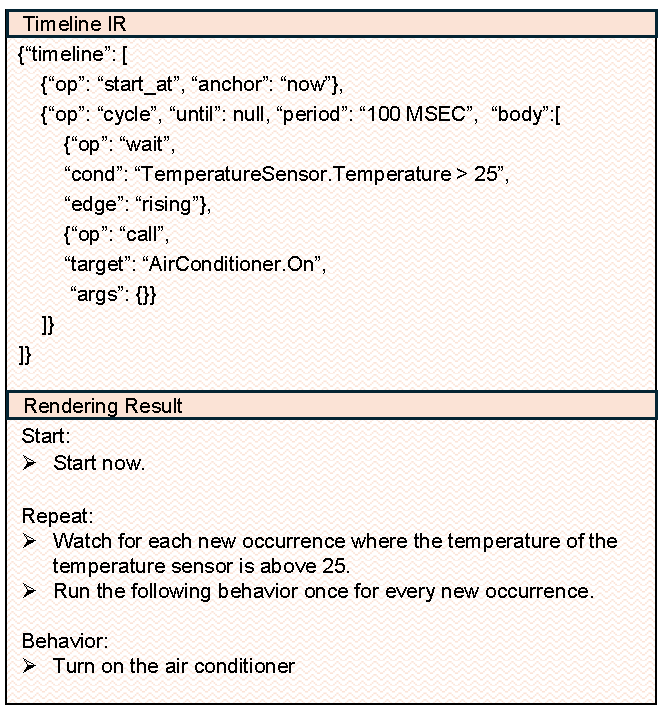
\includegraphics[width=\linewidth]{figs/rendering1.pdf}\par
\small (a) Recurring edge trigger
\end{minipage}\hspace{0.04\textwidth}%
\begin{minipage}[t]{0.42\textwidth}
\centering
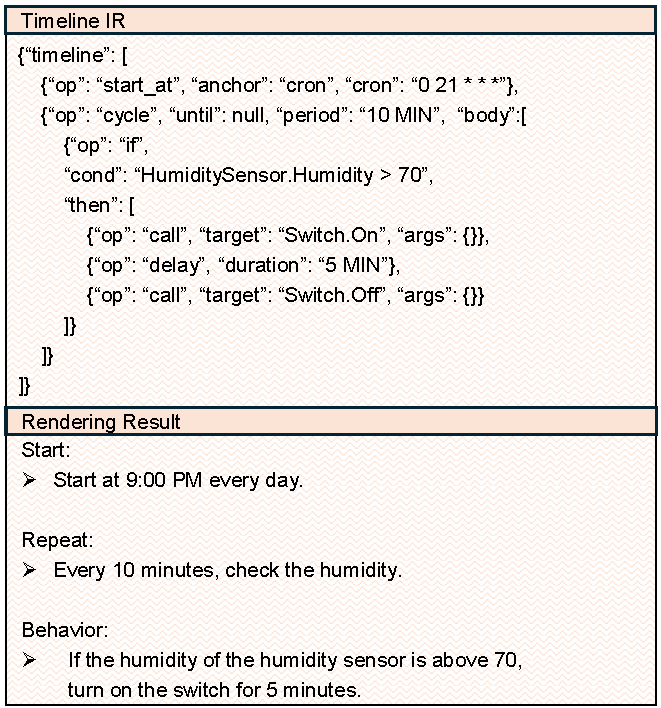
\includegraphics[width=\linewidth]{figs/rendering2.pdf}\par
\small (b) Scheduled periodic check with branch and delay
\end{minipage}
\caption{Two Timeline IRs and their deterministic plain-language renderings.}
\label{fig:ir}
\end{figure*}

\section{Timeline IR}

Timeline IR serves as the critical artifact connecting user confirmation to deterministic verification. %It has two roles. First, it is the source of the deterministic rendering shown to the user for approval. Second, once approved, it is the machine-checkable behavioral reference used by the verifier. 
While the NL→IR translation relies on an LLM, the IR→rendering process does not. Because the latter is a deterministic transformation, the text presented to the user is a faithful representation of the underlying IR that will subsequently be verified. % It is a deterministic transformation, so the text shown to the user is a faithful view of the IR that will later be checked. 
The rendering cannot introduce behavior absent from the IR, nor omit behaviors contained within it. %and it cannot hide behavior that the IR contains. 
In this sense, what is displayed is what is checked. The Timeline IR grammar is summarized in the appendix. 

\textbf{Closed control dimensions and primitive ops.} %These two roles are possible because 
The control dimensions of a reactive-temporal automation are limited and enumerable. A user command may specify the following dimensions: when the automation starts (\texttt{start\_at}), how often it repeats (\texttt{cycle.period}), what trigger or condition it waits for (\texttt{wait}'s condition and edge, or \texttt{if}'s condition), what action to perform and with what arguments (\texttt{call}), how long to wait or delay (\texttt{wait.for}, \texttt{delay}), and how to count or stop repeated behavior (\texttt{cycle.count}, \texttt{break}). Timeline IR maps primitive operations to these distinct dimensions, places the named slots directly on a timeline.

This representation is intentionally minimal. It avoids requiring the user to approve arbitrary code or write formal properties. %It does not ask the user to approve arbitrary code or write formal properties. 
Instead, the deterministic rendering exposes a bounded set of control slots specified by the command, ordered precisely as the behavior unfolds. User approval is therefore a closed judgment over those explicit slots: whether the displayed start time, period, trigger, condition, action, duration, and repetition behavior match the intended automation. The same slots are also the ones the verifier consumes. Thus, the IR serves a dual purpose: as an intuitive approval surface through its rendering, and as a rigorous behavioral reference for validating the generated code. %the IR is both an approval surface through its rendering and a behavioral reference for checking generated code.
The structural syntax G defined below ranges exactly over this closed set of operations.

\textbf{Finite-state view.} Timeline IR models an automation as a finite set of obligations on a timeline. An obligation can manifest as a scheduled check, a wait whose condition must become true, a branch whose guard selects a path, a call that must be issued, or a cycle body that must repeat at the next period. The IR admits no recursion and no unbounded loops. It uses bounded timers, counters, branches, and cycles, so the verifier can enumerate the relevant obligations within its checking horizon. Timeline IR is not intended to be a full timed-automaton model-checking language. It provides a highly operational view that renders the target behaviors both finite and explicit. %It is an operational view that makes the behaviors to be checked finite and explicit.

\textbf{Typed tree and structural syntax G.} Structurally, an IR is a typed tree. A structural syntax G specifies which parent-child relationships and control structures are legal. For example, an IR has exactly one \texttt{start\_at} and at most one top-level cron schedule. A \texttt{cycle} cannot appear inside another \texttt{cycle.body}. The \texttt{then} and \texttt{else} blocks can appear only as children of an \texttt{if}. A \texttt{break} is legal only inside a \texttt{cycle}. A \texttt{cycle} must have a period; its \texttt{until} condition is optional, and if it is absent the cycle repeats within the verifier's bounded checking horizon (\S6).

Whether an IR satisfies these structural rules is deterministic to decide. The same pass over the typed tree also produces the IR's structural class, τ(IR), which records the combination of rules used by that IR. OVLA uses τ(IR) later to route lowering exemplars with matching structure (\S7). This structural class helps generation, but it does not affect the verifier's accept/reject decision.

\textbf{Feasibility gate.} The feasibility gate in \S4 checks the structural validity of the extracted IR against G. It runs immediately after IR extraction and before lowering. If the extracted IR contains a nested cycle, a second top-level cron, a misplaced \texttt{then}/\texttt{else}, or a \texttt{break} outside a cycle, the gate rejects it before any JoI code is generated. This decision is a structural decision, not an empirical result: the gate checks the IR against the rules of G by construction.

This gate does not prove that the IR captures the user's true intent. It only establishes that the IR is structurally supported by OVLA's execution and verification pipeline. If the LLM extractor silently changes an unsupported request into a different but legal IR, the feasibility gate will accept the legal IR with the wrong meaning. That residual semantic mismatch is intentionally left to user confirmation through rendering. %For this reason, the extractor is designed to transcribe the requested structure rather than to repair or simplify it silently.

The primitive operators comprise \texttt{start\_at}, \texttt{wait} (condition, edge, and sustain duration), \texttt{delay}, \texttt{read}, \texttt{call}, \texttt{if} (then/else), \texttt{cycle} (period, count, until, and body), and \texttt{break}. Figure~\ref{fig:ir} illustrates this design with two Timeline IR examples and their deterministic renderings. Each example shows how internal IR slots map directly onto user-facing approval text.

Figure~\ref{fig:ir}(a) revisits the temperature example from \S1. The phrase ``whenever the temperature rises above 25°C'' is formalized into a \texttt{wait} operator whose condition is \texttt{Temperature > 25} and whose edge is rising, placed inside a \texttt{cycle}. The rendering exposes this edge slot to the user as ``each new occurrence'' and the \texttt{call} operator as ``Turn on the air conditioner.'' Figure~\ref{fig:ir}(b) shows a schedule-driven automation. The \texttt{start\_at} cron is rendered as ``Start at 9:00 PM every day,'' the \texttt{cycle.period} slot is rendered as ``Every 10 minutes,'' and the \texttt{if}-\texttt{call}-\texttt{delay}-\texttt{call} sequence is rendered as one conditional behavior. Even an empty \texttt{else} branch is rendered as ``Otherwise, do nothing.'' This is deliberate, ensuring that the rendering step neither drops nor adds behavior-relevant slots, a property \S8.1 measures exhaustively over 1,504 behaviorally different IR pairs.

\section{Verifier}

\subsection{Observation Model: Transition-Boundary Conformance}

The gate decides a single question: does the generated JoI code \emph{exhibit the same behavior} as the approved IR? As observed in \S2, the execution DSL has no primitives for the IR's control dimensions, so the LLM realizes each IR behavior as an idiom. For instance, ``sustained for $N$ minutes'' is implemented as a counter that increments on each poll tick and fires upon reaching a threshold. Similarly, ``edge (whenever)'' becomes a triggered flag set on firing and reset when the condition clears (or a prev/curr comparison), while ``every N minutes'' becomes periodic re-execution of the body. One IR behavior thus appears as several valid idioms and as countless near-misses one tick or one comparison off (Figure~\ref{fig:idiom}). This idiom-realization point is exactly where bugs enter. Equivalence must therefore be decided based on execution behavior (traces), not on syntax.

OVLA does not attempt to prove equivalence over every possible environment trace. Instead, it checks the points at which reactive-temporal behavior can change. These transition points include guard thresholds, condition edges, time landmarks such as delays and periods, and internal state transitions. Internal state transitions are changes in the program's own persistent state, such as a triggered flag being set or reset, a sustain counter reaching its firing threshold, or a cycle counter reaching the value that causes a break. They must be included because the same sensor value can lead to different behavior depending on the internal state: for example, the flag-based implementation in Figure~\ref{fig:idiom}(b) may fire before the flag is set and stay silent afterward.

The checked space is finite for two reasons. First, Timeline IR admits only bounded control: no recursion and no unbounded loops, so the reachable internal states within a run are finite. Second, the verifier uses a bounded time horizon. In our implementation, the verifier simulates one week, which contains a full recurrence of every time-of-day and day-of-week schedule. Calendar fields such as day-of-month and month do not require longer simulation. They only select on which dates the weekly pattern is active; they do not change the behavior inside that active window. The verifier therefore statically checks that the IR and the JoI code name the same calendar dates, and then reuses the already-simulated weekly behavior.

We call this observation model \textbf{transition-boundary conformance}. Under this model, two programs conform if their action traces agree, within the verifier's tolerance, at the boundaries where behavior can change: threshold crossings, condition edges, timer expirations, and next-cycle restarts, over the fixed bounded horizon. This is a boundary-focused equivalence judgment, not a proof over the entire input space. The restriction is deliberate. It makes the check deterministic, solver-free, and small enough to run on the edge hub. The verifier should therefore be read as a deployment-time filter, not as a replacement for heavyweight formal verification.

\subsection{Boundary Event Synthesis}

The event synthesizer is deterministic and LLM-free. It starts from the approved IR and derives an FSM that records which IR operations are active at each point in the execution. Each primitive operation contributes an obligation: \texttt{call} contributes an action obligation, \texttt{wait} and \texttt{delay} contribute temporal obligations, \texttt{read} contributes a value-observation point, \texttt{if} contributes guarded branches, and \texttt{cycle} and \texttt{break} contribute iteration and termination structure. Sequencing between operations imposes order, branches add guards, and cycles add the obligation to repeat the body at the next period.

The synthesizer's goal is to create concrete events for the boundaries identified by the observation model. For a rising-edge condition such as \texttt{wait(Temperature > 25, edge: rising)}, a boundary is the moment when the temperature changes from at most 25°C to above 25°C. For a \texttt{delay}, the boundary is the time when the delay expires. For a \texttt{cycle}, the boundary is the start of the next period.

These boundary events cannot be placed arbitrarily. The same temperature crossing matters only if the automation has already reached the \texttt{wait(Temperature > 25, edge: rising)} operation. It is not useful before earlier waits or delays have completed, on a branch that was not selected, or in a cycle iteration that has not been reached.

The synthesizer therefore needs to know where the automation is in its execution. It must know which waits and delays have completed, which branch was selected, which cycle iteration is active, and which IR operation is currently enabled. The FSM records this execution state explicitly.

Using this FSM state, the synthesizer places each representative event at a time when the corresponding IR operation is active and able to change the trace. Within a cell, the exact value crossed is not the important part; the timing and reachability of the event are. When a mismatch is found, the verifier attributes it to the obligation associated with that boundary, and that attribution becomes the counterexample returned to the repair loop of \S4.

The synthesis is based on IR semantics rather than JoI surface syntax. It tracks read→sensor flows and seeds both ends of each relevant value domain, so scale and offset mistakes can be exposed. For expressions that read the same sensor twice and compare the results, it additionally seeds the relation between the two reads in three directions—equal, rising, and falling—so sign and direction mistakes are exercised. Some IR arithmetic helpers, such as \texttt{abs}, \texttt{min}, and \texttt{max}, have no direct JoI counterpart. Lowering therefore expands them into conditional code, and the synthesizer seeds the internal boundaries of those expansions as well. This prevents, for example, an inverted clamp from passing simply because only ordinary threshold values were tested. The synthesizer also includes second-edge scenarios, where a condition clears and later becomes true again, because those cases are necessary to test whether the trigger can fire again after the condition clears. Read-modify-write accumulators are excluded from this targeted boundary seeding and are treated as a residual limit of the check. The final synthesized event set is fed unchanged to both the IR simulator and the JoI simulator, so the two artifacts are compared on identical inputs.

\subsection{Trace-Equivalence and Omission Detection}

The two simulators run on the same synthesized events and produce action traces. The verifier groups and deduplicates actions within a timing tolerance that absorbs tick quantization and the lowering's choice of polling period. Subsequently, it compares the traces sequentially, preserving % and then compares the traces in order. This preserves
behavior-relevant differences in action order, multiplicity, and boundary timing while avoiding verdict changes caused only by harmless polling-level timing variation.

This trace comparison detects both commission and omission. A commission error occurs when the JoI code performs an action that the IR does not allow. An omission error occurs when the IR requires an action and the JoI code fails to produce it. %The key point is that 
Significantly, silence is part of the trace. If the IR trace contains an empty interval, that interval is an oracle saying that no action should occur there.

This is why OVLA compares the JoI trace against the expected action trace produced by simulating the approved IR. The IR simulator does not only produce the actions that should happen; by producing no action during a time interval, it also specifies that the interval should remain silent. For example, if the approved IR says ``when the door opens, turn on the light after 5 minutes,'' the IR trace contains no action during the five-minute delay and then contains \texttt{Light.On()} at the end of the delay. Code that turns on the light immediately may reach the same final device state, but its JoI trace contains an action inside an interval where the IR trace is silent. Trace-equivalence detects this timing mismatch.

\subsection{What the Verdict Guarantees}

The verifier yields a deterministic, LLM-independent verdict. It provides two properties:
%The verdict is deterministic and LLM-free.
\begin{itemize}
\item \textbf{Determinism(T1)}: the same approved IR and generated JoI code always produce the same verifier verdict. 
\item \textbf{Rejection-Soundness(T2)}: when the verifier rejects a program, it has found a real trace mismatch under the observation model defined above. In other words, rejection is tied to an executable counterexample, not to a probabilistic judgment.
\end{itemize}

We do not claim absolute correctness upon passing (``pass ⇒ correct''). A pass means only that the generated code matches the approved IR on the synthesized boundary traces within the bounded horizon and tolerance. The trusted computing base is strictly confined to the deterministic verifier: the IR simulator, the JoI simulator, the tolerance policy, and the trace-equivalence relation. The verdict therefore does not rely on trusting the LLM that generated the code. The soundness of a rejection reduces to simulator fidelity rather than to a proof over all environments. We evaluate the check empirically in two ways: \S8.2 stress-tests verifier detection and the adequacy of the synthesized traces with construct-derived mutation tests and coverage measured on both the IR-FSM obligations and the generated JoI branches, and \S8.3 measures the deployment outcome of applying the gate to generated automations. Surviving mutants are characterized individually.

\subsection{Limits of the Check}

The limitations of the check stem directly from the observation model. First, the one-week horizon, together with the static calendar check, covers time-of-day and day-of-week schedule behavior. It does not exercise behaviors whose own duration exceeds the horizon, such as a month-long sustained condition, to completion. Such automations can still be represented, but their long-duration behavior is outside the exercised region.

Second, the check is limited by arithmetic lacking explicit boundaries.
%The second limit is arithmetic without a boundary. 
The three-direction relational seeding of \S6.2 exercises sign and direction errors, but an expression whose value flows into an argument, such as \texttt{notify(\$t1-\$t2)}, defines no threshold, edge, or timer at which the synthesizer can target a representative boundary. Consequently, value-specific bugs dependent on precise numerical relations may survive, even though generic seeds can still detect sign errors or structural flaws.
%Generic seeds can still expose sign errors or structural mistakes, but value-specific bugs that occur only under particular numeric relations can survive. 
These limits do not make the two simulators disagree about the same input; rather, they identify places where the synthesized event set may fail to exercise a bug.

\section{Implementation}

OVLA's deterministic core is pure Python with no external dependencies. The two simulators (about 3.7K lines), the verifier (1.1K), the rendering (0.7K), and the feasibility gate (0.1K) total roughly 5.7K lines of deterministic code, with no solver and no model call. Generation runs on off-the-shelf 4-bit-quantized models of at most 9B parameters, without fine-tuning (\S8 Setup). Generation is decomposed into the stages of \S4 (intent analysis, device and tool mapping, IR extraction, lowering), and the verifier's guarantee is independent of which generator produces the code.

\textbf{Structure-based example routing.} The lowering prompt does not carry few-shot examples for every idiom family. Instead, OVLA reuses the structural class of the IR determined by the feasibility pass (\S5), and the prompt includes only the lowering examples for that class, which keeps the prompt small enough for a local model. On our dataset, this routing reduces the lowering prompt by 33\% on average compared with carrying every class's examples (38\% for acyclic IRs, 19\% for cyclic ones). We use this number only as an implementation-cost measurement: routing reduces prompt length and therefore memory/context pressure on the local model. After a generated pair passes the verifier, the corresponding (IR, JoI) pair can be stored under its structural signature; if a failed lowering is repaired and later passes, the repaired pair becomes an example for future requests of the same class. This routing affects only the generator's prompt. The accept/reject verdict remains the deterministic check of \S6. We do not claim that routing improves lowering accuracy, and we do not ablate it as an accuracy factor in this submission.

\section{Evaluation}

Our evaluation asks four questions, ordered as the pipeline reaches the user. Does the rendering the user approves faithfully display the IR (\S8.1)? Taking the approved IR as the reference, does the verifier catch wrong code (\S8.2)? Does the full pipeline, with the verifier as its gate, classify generated code correctly (\S8.3)? And is all of this affordable on an edge device (\S8.4)? Each answer is a premise for the next: every later check takes the user-approved IR as its reference, and the interpretation of the gate's outcomes rests on the verifier's detection quality.

\textbf{Setup.} \emph{Hardware and models}: the primary edge device is a Mac mini M4 (16GB). Experiments that require many model generations run on GPU servers, while all on-device cost measurements run on the M4. Generation uses Qwen3.5-9B, with Qwen3-8B and Gemma-4-E4B as additional generators (Table~\ref{tab:models}); all are 4-bit quantized without fine-tuning. The deterministic verifier runs identically across backends.

\emph{Dataset}: the benchmark contains 382 natural-language automation commands over 24 device/service categories supported by the target platform. We wrote the commands to cover the reactive idiom families that commonly cause lowering errors in JoI—triggers, rising and falling edges, sustained conditions, periodic checks, delayed sequences, branches, and bounded counting—and did not curate them to fit OVLA's IR schema. Each command is paired with a manually authored reference Timeline IR, independently audited at the value level: start times, periods, trigger edges, sustain and delay durations, branch conditions, target services, and action arguments were checked against the source command. The category breakdown is reported in the appendix.

\emph{Metrics}: one per question—rendering faithfulness (the fraction of behaviorally different IR pairs that render as different text), verifier detection (mutation catch rate and scenario coverage), gate classification accuracy (full audit and independent re-examination), and on-device cost (latency distribution, memory, and power).

\subsection{RQ1: Rendering Faithfulness}

In OVLA the user approves an automation by reading the rendering of its IR, not its code, and every later check takes that approved IR as its reference. As \S5 showed, Timeline IR expresses an automation's behavior through a finite set of control slots—start time, period, trigger condition and edge, action and arguments, sustain and delay durations, repetition and termination—and the rendering unfolds those slots into plain language in timeline order. We therefore show, with the experiment of Table~\ref{tab:faithful}, that \emph{every behavioral difference this finite slot set can produce is displayed to the user as different plain text}. If even one slot difference rendered identically, the user could not tell a wrong IR from the right one, and the gate would then check against the wrong reference.

\textbf{Design.} We measure in two parts. The synthetic check (Part A) takes each of the 382 reference IRs and injects eight fault classes, each twisting one dimension of the slot set—comparator flips, polarity inversions, and AND-conjunct drops on condition slots; argument values and target devices on action slots; durations on time slots; oneshot↔wait-until and single↔cycle on structure slots—at every applicable slot, producing 1,504 (correct, faulty) IR pairs, and compares the two renderings of each pair. The judgment is deterministic: if the two rendered texts differ, the fault is surfaced; if they are identical, it is blind. The real-fault check (Part B) injects nothing: it takes the 55 logic-faulty IRs that NL→IR extraction (Qwen3.5-9B) actually produced and that passed the static validation gates to reach rendering, and compares them against the reference IRs' renderings in the same way. Part A measures exhaustive coverage of the fault space we defined; Part B confirms that this fault design holds on the error distribution a real LLM produces.

\textbf{Results.} All 1,504 synthetic pairs surfaced as distinct text, with zero blind spots (Table~\ref{tab:faithful}). The result holds on real logic faults: all 55 surfaced. For example, in the oneshot↔wait-until class the correct IR renders as ``If the charging state of the charger is fullyCharged, turn off the selected switch.'' while the faulty IR renders as ``Wait until the charging state of the charger is fullyCharged is true. Turn off the selected switch.''

\begin{table}[t]
\centering
\caption{Rendering faithfulness: do behaviorally different IR pairs render differently?}
\label{tab:faithful}
\small
\begin{tabular}{lrr}
\toprule
Fault class & n & Surfaced (\%) \\
\midrule
comparator                & 267 & 100 \\
polarity                  & 85  & 100 \\
wrong arg value           & 235 & 100 \\
wrong device              & 382 & 100 \\
timing/duration           & 74  & 100 \\
oneshot↔wait-until        & 150 & 100 \\
single↔cycle (whenever)   & 273 & 100 \\
AND-conjunct drop         & 38  & 100 \\
\midrule
Synthetic total (Part A)   & 1,504 & 100 \\
Real logic faults (Part B) & 55  & 100 \\
\bottomrule
\end{tabular}
\end{table}

\subsection{RQ2: Verifier Detection}

Having established that the approval surface is faithful, we turn to the verifier itself, which checks generated code against the approved IR. The question is simple: does the verifier actually catch wrong code? To measure this we detach the verifier from the deployment pipeline and plant controlled faults in correct code. What happens when this verifier gates the full system is the subject of RQ3.

\textbf{Mutation.} Measuring detection requires a large supply of code that is correct except for one slip. The experiment therefore proceeds as follows. We take the 328 (IR, correct code) pairs that pass the verifier as seeds. From each seed we twist exactly one spot of the correct \emph{code}—numeric argument changes, enum swaps, call deletions and insertions, tick scaling, guard polarity flips, comparator swaps: twelve operators in total (Table~\ref{tab:mutation}). We then feed each mutant, together with the original IR, to the verifier. A rejection means the fault is caught; a pass means it is missed (a survivor). Where RQ1 twisted the IR and asked whether the rendering exposes the difference, here we twist the code and ask whether the verifier catches it.

We do not choose the number of mutants: every applicable site gets one first-order mutant, so the site count is the mutant count (e.g., 436 call sites yield 436 \texttt{call\_drop} mutants). This generates 1,651 mutants (Gen.); excluding 99 equivalent mutants whose traces match the original under every scenario (Equiv.)—for example, changes on unreachable branches—leaves 1,552 genuine mutants (Genuine), of which the verifier catches 1,541, or 99.3\% (Caught).

Only three operators in Table~\ref{tab:mutation} fall short of 100\%, and none of the 11 survivors is a new weakness. Eight (\texttt{comparator}) replace \texttt{>=} with \texttt{>} on a sustain counter; the entire effect is that the action fires one tick (100ms) late, inside the timing tolerance that exists precisely to absorb normal polling-time slack, so passing is the intended design. One (\texttt{call\_drop}) deletes one of two identical commands sent to two rooms at the same instant; whether the command is sent once or twice, the final device state is the same, so no distinguishing point remains in the deduplicated trace. The remaining two sit in a single read-modify-write arithmetic automation that \S6.2 excludes from boundary seeding—the residual class we already disclosed, appearing where expected.

\textbf{Coverage.} All of this detection happens on the synthesized event scenarios of \S6.2, so we separately measure whether those scenarios reach every check point (Table~\ref{tab:coverage}). A check point is a place the scenarios could fail to visit depending on how inputs are seeded: both the then and else sides of every \texttt{if}, the edge and sustain of every \texttt{wait}, and the value boundaries of every arithmetic expression. \texttt{call}, \texttt{delay}, and \texttt{cycle} are exercised unconditionally once execution reaches them and are checked by the trace comparison itself, so they are not counted here. The scenarios reach 97.5\% (350/359) of these points. All 9 unreached points are the else side of modulo guards over a cycle's iteration counter (\texttt{n \% k == c}): the counter is not a sensor, so no seeded value can steer it. Measuring the same scenarios on the generated JoI code, 97.7\% (676/692) of the code's own branches actually execute—the scenarios do not just walk the spec; they reach inside the code under test.

A caution in reading the 99.3\%: the operators that make mutants and the verifier's check points are both derived from the same list of IR constructs. The number therefore says that the verifier catches the kinds of faults it was designed to catch; it does not vouch for bugs outside that list. We do not claim ``pass ⇒ correct'' (\S6.4).

\begin{table}[t]
\centering
\caption{Construct-derived mutation results (328 seeds, 12 operators).}
\label{tab:mutation}
\small
\setlength{\tabcolsep}{4.5pt}
\begin{tabular}{lrrrr}
\toprule
Operator & Gen. & Equiv. & Genuine & Caught (\%) \\
\midrule
arg\_numeric    & 142 & 1  & 141 & 141 (100) \\
enum\_flip      & 111 & 2  & 109 & 109 (100) \\
call\_drop      & 436 & 4  & 432 & 430 (99.5) \\
call\_add       & 200 & 3  & 197 & 197 (100) \\
tick\_scale     & 55  & 0  & 55  & 55 (100) \\
guard\_polarity & 198 & 0  & 198 & 198 (100) \\
comparator      & 159 & 34 & 125 & 117 (93.6) \\
assign\_init    & 71  & 13 & 58  & 58 (100) \\
cmp\_direction  & 159 & 30 & 129 & 128 (99.2) \\
arith\_op       & 37  & 7  & 30  & 30 (100) \\
break\_drop     & 29  & 5  & 24  & 24 (100) \\
wait\_drop      & 54  & 0  & 54  & 54 (100) \\
\midrule
Total           & 1,651 & 99 & 1,552 & 1,541 (99.3) \\
\bottomrule
\end{tabular}
\end{table}

\begin{table}[t]
\centering
\caption{Spec-side coverage of the synthesized scenarios: the fraction of IR-defined check points the scenarios actually reach.}
\label{tab:coverage}
\small
\begin{tabular}{lrrr}
\toprule
Obligation & Total & Covered & (\%) \\
\midrule
\texttt{if}: then branch            & 166 & 166 & 100 \\
\texttt{if}: else branch            & 37  & 28  & 75.7 \\
\texttt{wait} (edge/sustain/second edge) & 122 & 122 & 100 \\
arithmetic expr boundary (lo/hi/fall) & 34  & 34  & 100 \\
\midrule
Total                               & 359 & 350 & 97.5 \\
\bottomrule
\end{tabular}
\end{table}

\subsection{RQ3: System Safety}

Finally we run the full pipeline, with the verifier as its gate, on all 382 commands. The gate verifies each lowering candidate, deploys it if it passes, and otherwise enters a repair loop that returns the counterexample to the generator (at most two attempts), rejecting fail-closed if repair also fails. With the 9B generator the outcome distribution is: 347 deploy on the first candidate, 11 deploy after repair, and 24 are rejected.

This distribution is split by the gate's own verdict, so the question to ask is not the distribution but the \emph{accuracy of the classification}: does code classified as deployable really behave as the user-approved IR, and was code classified as rejected really divergent? We re-examined both directions independently.

\textbf{Rejection side: was rejected code really divergent?} We audited all 35 candidates the gate flagged (9.2\% of 382). 33 are genuine behavioral divergences (sustain mistimings, inverted logic, counter misuse, sign-ignoring arithmetic), and 2 are subset rejections of unparseable code. No correct program was rejected by mistake. Replaying the 22 simulatable rejections under randomized dense scenarios unrelated to the boundary synthesis reproduces the divergence in 19 of them (the remainder are of the kind that requires hitting a boundary precisely). Without the gate, these 35 would have deployed while silently diverging from the approved IR.

\textbf{Deployment side: does deployed code really match the IR?} We replayed every deployed (IR, code) pair under 100 randomized dense scenarios each—36,000 in total—and compared with the same criterion. To state the conclusion first: this re-examination confirmed that all 358 finally deployed automations match their IRs, and along the way it surfaced two real bugs in exactly the residual class disclosed in \S6.5 (variable-to-variable arithmetic). The two share one pattern: for an IR saying ``if the value rose by at least N,'' the code compares the unsigned absolute difference, so it also fires when the value \emph{falls}. The root cause was that the synthesizer of \S6.2 seeded the two read values only as equal or rising, never falling; we added a falling scenario, which makes this entire class deterministically detectable. Both bugs failed repair and were rejected fail-closed, and the numbers in this section are after this strengthening. In the post-strengthening re-examination, 356 of the 358 deployed automations matched on every scenario; the remaining two, unrelated to the bug above, showed only a phase offset in which a periodic lowering reacts up to one tick period late—behavior the tolerance design permits.

\textbf{Across generation models.} Repeating the same pipeline with two weaker generators produces up to 1.8$\times$ more divergent candidates, and the error rate is not monotone in model size, yet the classification accuracy holds: divergent candidates are repaired or rejected, and no divergent candidate was classified as deployable (Table~\ref{tab:models}). Because the gate is deterministic, this property does not depend on generation stochasticity. These numbers concern divergence from the approved IR, not whether the IR matched the user's true intent (Layer A; \S9).

\begin{table}[t]
\centering
\caption{Gate classification across generation models (382 automations, confirmed IR). Divergent = candidates flagged by the gate, confirmed by full audit.}
\label{tab:models}
\small
\setlength{\tabcolsep}{4pt}
\begin{tabular}{lrrrr}
\toprule
Generator (4-bit, no FT) & Divergent & Rep. & Rej. & Deployed \\
\midrule
Qwen3.5-9B  & 35 (9.2\%)  & 11 & 24 & 358 \\
Qwen3-8B    & 63 (16.5\%) & 11 & 52 & 330 \\
Gemma-4-E4B & 55 (14.4\%) & 16 & 39 & 343 \\
\bottomrule
\end{tabular}
\end{table}

\subsection{RQ4: On-Device Cost and Deployment}

The remaining question is whether all of this is affordable on an edge device. We report verification cost as a latency distribution with memory and power, and close with a live deployment on a physical testbed.

\textbf{On-device cost.} On the M4, the verifier checks one automation in 0.97ms at the median over all 382 automations (10 repetitions each), peaks at 54MB of memory, and never touches the GPU (5.5W CPU). The latency distribution is long-tailed (p95 0.7s, worst 8.4s): the tail is not structural complexity but one class whose specification itself acts on every tick (1-second level-triggered polling over the verification horizon), bounded by the tick cap. LLM cost is confined to the one-time authoring step (generation runs at 10.2W on the GPU), and a deployed automation makes zero LLM calls. Efficiency numbers are reported as the precondition for on-device deployment, not as a contribution in themselves.

\begin{figure}[t]
\centering
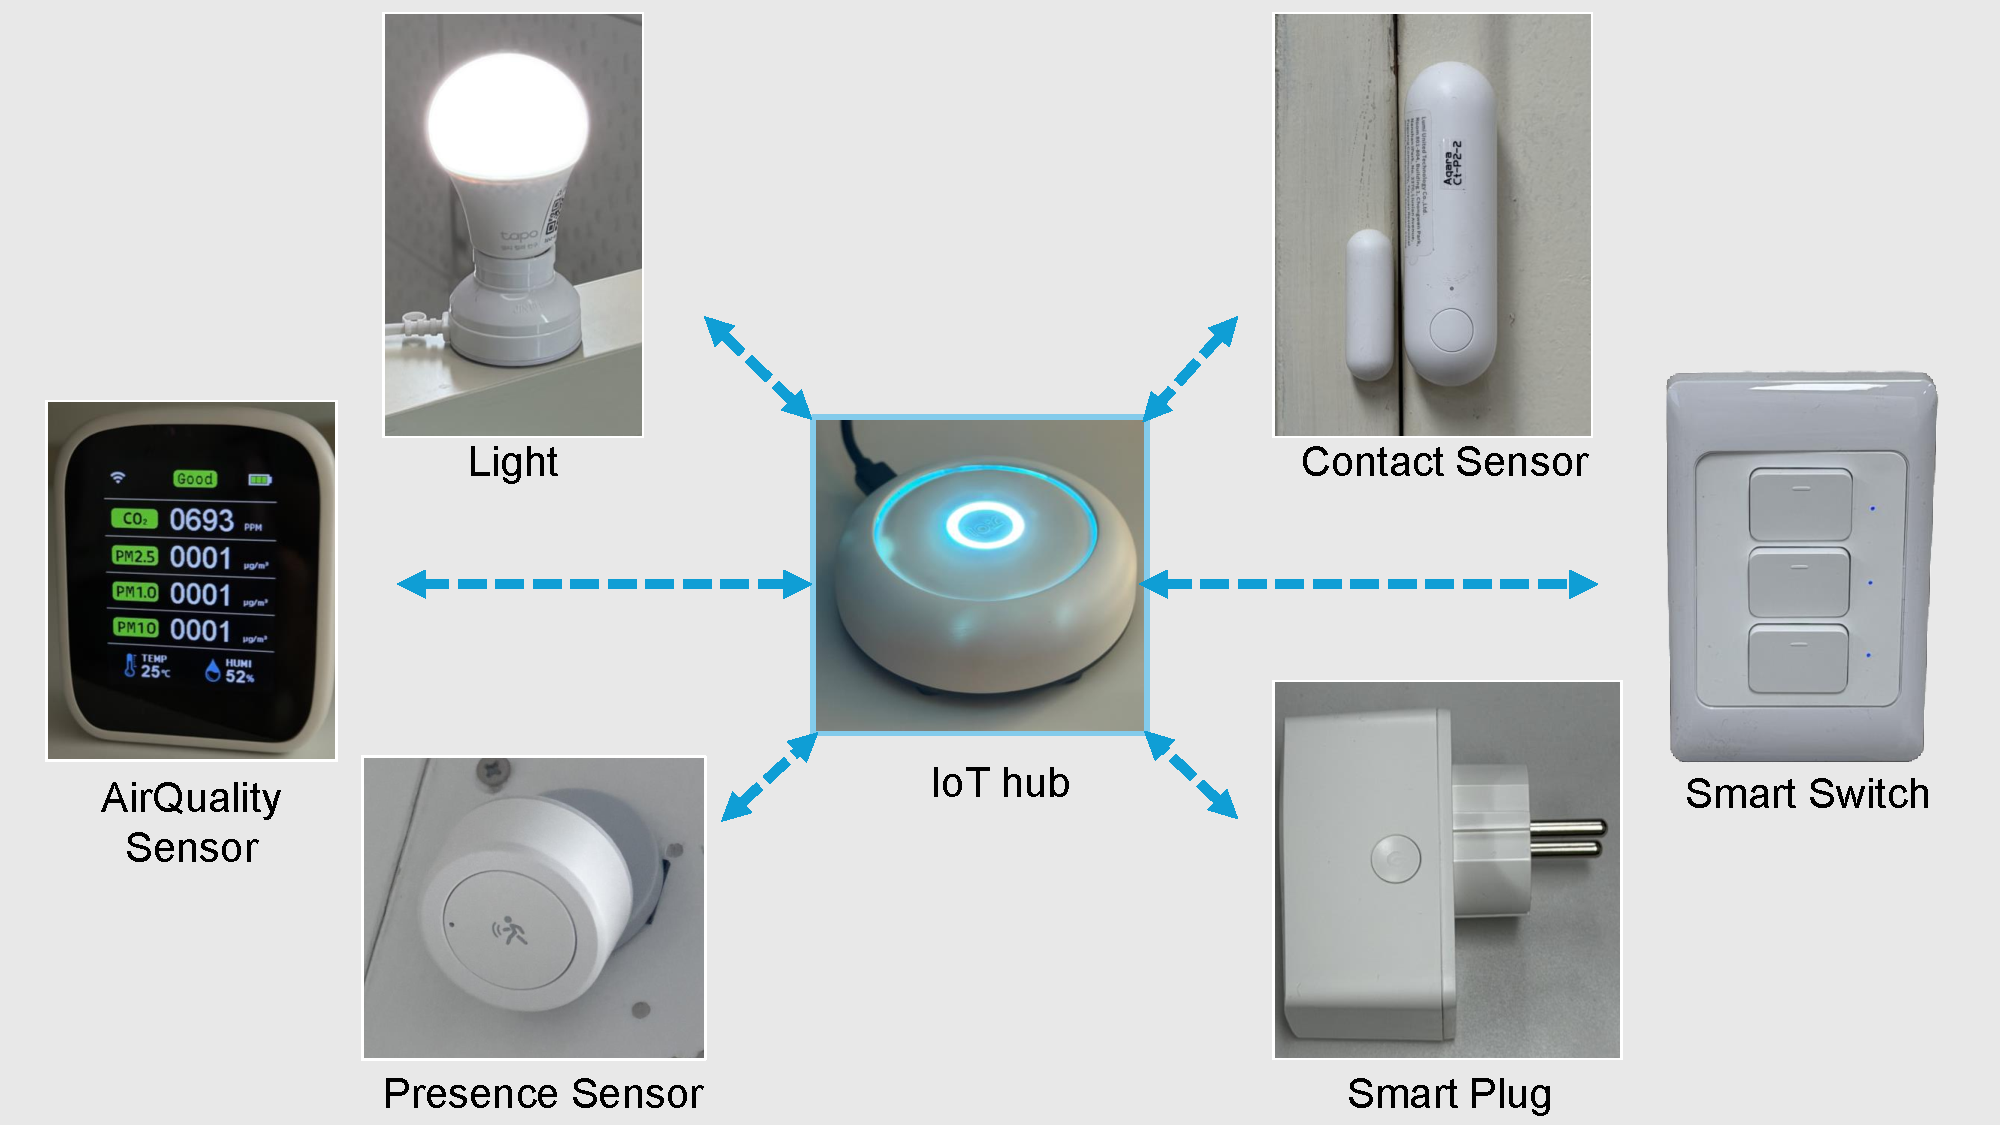
\includegraphics[width=.95\linewidth]{figs/Environment.pdf}
\caption{The physical testbed: a commercial edge hub with the sensors and actuators used in the deployment demonstration.}
\label{fig:testbed}
\end{figure}

\textbf{Deployment.} On a commercial home-automation platform (name withheld for review) with a Raspberry Pi based edge hub and physical devices (presence, contact, and air-quality sensors; plugs, lights, and a speaker; Figure~\ref{fig:testbed}), we authored six new commands live through the full pipeline (IR extraction, confirmation, lowering, gate) and registered the gate-approved lowerings. This is an existence proof, not statistics.

The representative automation, ``if no one is present in the meeting room for at least 5 minutes, turn off the TV plug,'' reproduced the sustain fault class naturally: all four ungated generations were divergent (firing after 30 or 3 seconds instead of 5 minutes), and five of six gated authoring sessions ended in fail-closed rejection before one session's repair produced a correct lowering. Figure~\ref{fig:rq4} shows the observed device behavior: without the gate the TV plug switches off 30 seconds after the room is vacated; with the gate, at 5 minutes, matching the IR-predicted trace.

Across the registered automations (edge trigger, counted cycle, delay sequence, and two rising-threshold automations), every observed action sequence matched the IR-predicted trace at the platform's logging resolution (Table~\ref{tab:deploy}), including the negative obligations (a counted cycle stopping after exactly 3 announcements; no re-announcement while a crossed threshold stays high). Authoring also exercised the upstream gates: two initial wordings produced a one-shot conditional IR whose rendering revealed the misreading at confirmation, and one produced an out-of-catalog target that was rejected fail-closed at extraction validation.

\begin{table}[t]
\centering
\caption{Live-authored automations on the physical testbed: gate outcome and predicted-vs-observed behavior.}
\label{tab:deploy}
\small
\setlength{\tabcolsep}{2.5pt}
\begin{tabular}{llll}
\toprule
Automation & Idiom & Gate & Observed \\
\midrule
presence absent 5min → TV plug off & sustain & repaired & off at 5:00 \\
speak every 30s, 3 times only & count & pass & 3 only, stops \\
door opens → light on & edge & pass & immediate \\
light off, on after 3min & delay & pass & on at 3:00 \\
CO\textsubscript{2} rises above 900 → announce & rising & pass & on crossing only \\
temp.\ rises above 28° → switch on & rising & pass & on crossing only \\
\bottomrule
\end{tabular}
\end{table}

\begin{figure}[t]
\centering

\includegraphics[width=.92\linewidth]{figs/deployment.pdf}
\caption{The representative automation on the physical testbed: without the gate, the naturally generated buggy lowering turns the TV plug off 30 seconds after the room is vacated; the gate-repaired lowering fires at 5 minutes, matching the IR-predicted trace.}
\label{fig:rq4}
\end{figure}

\section{Limitations}

The largest limitation is that NL→IR intent correctness remains open (Layer A). A user can approve a mis-displayed IR, in which case the verifier faithfully checks against the wrong spec. We do not study human confirmation behavior in this round; we establish only that the rendering is a deterministic, faithful plain-language surface. Ethics: no human-participant data was collected (``Not applicable: no human participants'').

Beyond that, the limits are: the coverage ceiling (the else side of counter-modulo guards; \S8.2); boundary-focused equivalence is not a whole-input-space guarantee, although the dense re-examination of \S8.3 measures this residual on the deployed set; the bounded 7-day horizon; continuous arithmetic (SMT as future work); arithmetic whose value flows into an argument, where value-specific bugs can survive (a coverage limit, not a soundness issue; \S6.5); two reads of the same service collapsing onto one device key in the selector-free IR (precision is outside this paper's scope); and generalization beyond one platform.

\section{Conclusion}

Reactive-temporal IoT automations have become easy to generate with LLMs, but the step that decides whether they are correct to deploy has been empty. OVLA confines the LLM to generation and makes the deployment gate deterministic and LLM-free: the user approves a plain-language rendering of the IR, a deterministic checker tests the generated code against that approved IR by bounded trace-equivalence, and divergent code is repaired or rejected fail-closed. Across 382 automations, every divergent candidate the generators produced (9.2\% for the strongest) was repaired or rejected rather than deployed, and the gate's classification survived independent re-examination on both sides — a full audit of the rejections and 36,000 randomized dense replays of the deployed set — with no LLM in the verification loop, on an edge device. OVLA does not solve natural-language intent correctness, but it removes the separate silent failure mode that survives user approval.

\balance
\bibliographystyle{ACM-Reference-Format}
\bibliography{refs}

\appendix

\section{Timeline IR Grammar}
\label{app:grammar}

A Timeline IR is serialized as a JSON object whose steps each carry an \texttt{op} tag; the grammar below gives the abstract syntax in EBNF. Terminals are quoted; \texttt{[\,x\,]} marks an optional part and \texttt{\{\,x\,\}} zero-or-more repetition.

{\small
\begin{flushleft}
\texttt{ir \ \ \ \ \ \ ::= start\_at \{ step \}}\\
\texttt{step \ \ \ \ ::= wait | delay | read | call}\\
\texttt{\ \ \ \ \ \ \ \ \ \ \ | if | cycle | break}\\[3pt]
\texttt{start\_at ::= "start\_at" "(" ("now" | "cron" cron) ")"}\\
\texttt{wait \ \ \ \ ::= "wait" "(" expr ["," "edge:" edge]}\\
\texttt{\ \ \ \ \ \ \ \ \ \ \ \ \ ["," "for:" duration] ")"}\\
\texttt{edge \ \ \ \ ::= "none" | "rising" | "falling"}\\
\texttt{delay \ \ \ ::= "delay" "(" duration ")"}\\
\texttt{read \ \ \ \ ::= "read" "(" ident "," service "." attr ")"}\\
\texttt{call \ \ \ \ ::= "call" "(" service "." function}\\
\texttt{\ \ \ \ \ \ \ \ \ \ \ \ \ \{ "," name "=" (value | expr) \} ")"}\\
\texttt{if \ \ \ \ \ \ ::= "if" "(" expr ")" "\{" \{ step \} "\}"}\\
\texttt{\ \ \ \ \ \ \ \ \ \ \ \ \ ["else" "\{" \{ step \} "\}"]}\\
\texttt{cycle \ \ \ ::= "cycle" "(" "period:" duration}\\
\texttt{\ \ \ \ \ \ \ \ \ \ \ \ \ ["," "count:" ident]}\\
\texttt{\ \ \ \ \ \ \ \ \ \ \ \ \ ["," "until:" expr] ")"}\\
\texttt{\ \ \ \ \ \ \ \ \ \ \ \ \ "\{" step \{ step \} "\}"}\\
\texttt{break \ \ \ ::= "break"}\\[3pt]
\texttt{duration ::= int ("HOUR" | "MIN" | "SEC" | "MSEC")}\\[3pt]
\texttt{expr \ \ \ \ ::= expr ("or" | "and") expr | "not" expr}\\
\texttt{\ \ \ \ \ \ \ \ \ \ \ | arith [cmp arith]}\\
\texttt{cmp \ \ \ \ \ ::= "==" | "!=" | "<" | "<=" | ">" | ">="}\\
\texttt{arith \ \ \ ::= arith ("+" | "-" | "*" | "/") arith}\\
\texttt{\ \ \ \ \ \ \ \ \ \ \ | "abs" "(" expr ")"}\\
\texttt{\ \ \ \ \ \ \ \ \ \ \ | ("min" | "max") "(" expr "," expr ")"}\\
\texttt{\ \ \ \ \ \ \ \ \ \ \ | service "." attr | "\$" ident | literal}
\end{flushleft}
}

\noindent\texttt{service.attr} denotes a live sensor read and \texttt{\$}\texttt{ident} a persistent variable bound by \texttt{read} or \texttt{cycle.count}; \texttt{literal} ranges over numbers, booleans, and the enum values declared in the device catalog.

\noindent\emph{Semantic conventions.} \texttt{wait.edge="rising"} completes once per upward crossing of \texttt{cond}; \texttt{wait.for} requires \texttt{cond} to hold continuously for the duration, resetting if it flips false. \texttt{cycle.period} is the per-iteration cadence; when \texttt{until} is absent, the cycle repeats within the verifier's bounded horizon (\S6).

\noindent\emph{Context-sensitive rules (grammar G, \S5).} Beyond per-step shape, the feasibility gate enforces: (1) \texttt{timeline[0]} is the only \texttt{start\_at}; (2) \texttt{start\_at} may not appear inside a branch or loop body; (3) at most one top-level \texttt{cycle} and no nested \texttt{cycle}; (4) \texttt{break} only inside a \texttt{cycle} body; (5) \texttt{cycle.period} is required. Catalog conformance (every \texttt{Service.Attr} and \texttt{call.target} names a service, member, and argument that the connected-device catalog declares) is checked at the same point and rejects out-of-catalog targets fail-closed.

\section{Dataset Category Breakdown}
\label{app:categories}

Table~\ref{tab:categories} reports the 24-category breakdown of the 382-command benchmark. Each category corresponds to a structurally distinct reactive pattern and its lowering idiom.

\begin{table}[h]
\centering
\caption{Dataset categories (382 commands, 24 categories).}
\label{tab:categories}
\small
\setlength{\tabcolsep}{4pt}
\begin{tabular}{llr}
\toprule
ID & Pattern & n \\
\midrule
C01 & Single device action & 28 \\
C02 & Action with device selector & 33 \\
C03 & Single-condition \texttt{if} (incl.\ if-else) & 34 \\
C05 & AND-compound \texttt{if} & 30 \\
C06 & OR-compound / chained \texttt{if-elif-else} & 7 \\
C07 & Level-triggered wait (``when X, do Y'') & 32 \\
C08 & Rising-edge trigger (``whenever'') & 41 \\
C09 & Sequential delay & 18 \\
C10 & Trigger + delayed action & 9 \\
C11 & Snapshot, delay, and re-read comparison & 8 \\
C12 & Phase lifecycle (``when X, every N thereafter'') & 15 \\
C13 & Alternation / binary toggle & 7 \\
C14 & Progressive update with counter and stop & 7 \\
C15 & Cron-scheduled action & 21 \\
C16 & Cron + branch & 13 \\
C17 & Periodic polling + branch & 12 \\
C18 & Bounded duration (time-window cycle) & 10 \\
C19 & Hysteresis (double-threshold deadband) & 8 \\
C20 & Sustained condition (``for at least N'') & 17 \\
C21 & Group consensus (all/any quantifier) & 7 \\
C22 & Counted repetition (``repeat N times, stop'') & 10 \\
C23 & Sustained trigger + multi-step sequence & 5 \\
C24 & Sustained trigger + repeating alert & 5 \\
C25 & Periodic polling + if-else & 5 \\
\midrule
 & Total & 382 \\
\bottomrule
\end{tabular}
\end{table}

\end{document}
